\section{Experiments}

Up until now, protocols and cloud background were discussed. These backgrounds serves as a way to understand the decisions taken during experiments in the following sections.

This section explains the reasons for each experiment's characteristics, why each scenario is considered, what they bring to the table, and what kind of metrics are going to be collected.

\subsection{Objectives}

These experiments have the objective to compare QUIC with other transport-layer protocols: \gls{udp}, \gls{tcp}, and \gls{tcp}+\gls{tls}. Their results are going to make assessments about each transport-layer protocol performance and resource efficient use. Therefore, latency, throughput, and CPU and memory usage metrics are going to be collected.

Furthermore, to be able to observe QUIC's influence on a production environment, they have the objective to compare HTTP/3 with other application-layer protocols: HTTP/1, HTTP/1+\gls{tls}, HTTP/2, and HTTP/2+\gls{tls}. Their results are going to make assessments about each application-layer protocol performance and resource efficient use. Therefore, latency, throughput, and CPU and memory usage metrics are also going to be collected.

\subsection{Preparation}

This subsection explains what kind of preparations were made to be able to experiment on protocols. This includes how the benchmark service was implemented, where it was deployed and what kind of scenarios its trying to simulate. 

\subsubsection{Benchmark Service}

The benchmark service was developed to be able to experiment with each protocol. Their impact on performance and resource usage are analyzed by collecting metrics about latency, throughput, and CPU and memory usage. Therefore, it was developed in the most efficient way possible to avoid any external noises that might pollute the results.

Google's QUIC experimentations paper refers \textit{lucas-clemente/quic-go}'s QUIC implementation as being one the ones that provided invaluable feedback \cite{quic_protocol}. Therefore, the benchmark service was implemented in Go and uses this library on QUIC's and HTTP/3's experiments.

This implementation took into consideration three types of clients: ephemeral, sequential persistent, and parallel persistent clients. By separating clients into these three categories, experiments are able to simulate three very common scenarios on distributed systems and observe how QUIC behaves when having to deal with each one of them.

The first scenario explores ephemeral connections. It represents a job that needs to perform some sort of finite task, creating a single connection to the server, and closing it once it’s done.

The second scenario explores sequential persistent connections. It represents a service that needs to communicate with a database to provide some kind of functionality, creating a single connection to the database throughout its entire lifetime and performing one request at a time.

The third and final scenario explores parallel persistent connections. It represents a service similar to the previously explained. However, it can perform multiple requests at the same time.

Metrics are collected through two different measurements. The first uses the \textit{time} command to get information about CPU time, memory usage and wall clock time as seen in Figure \ref{fig:time_command}. The second uses the benchmark service's logs to calculate latency and throughput. These logs are the time each request took to receive its response.

\begin{figure}[h!]
    \centering
    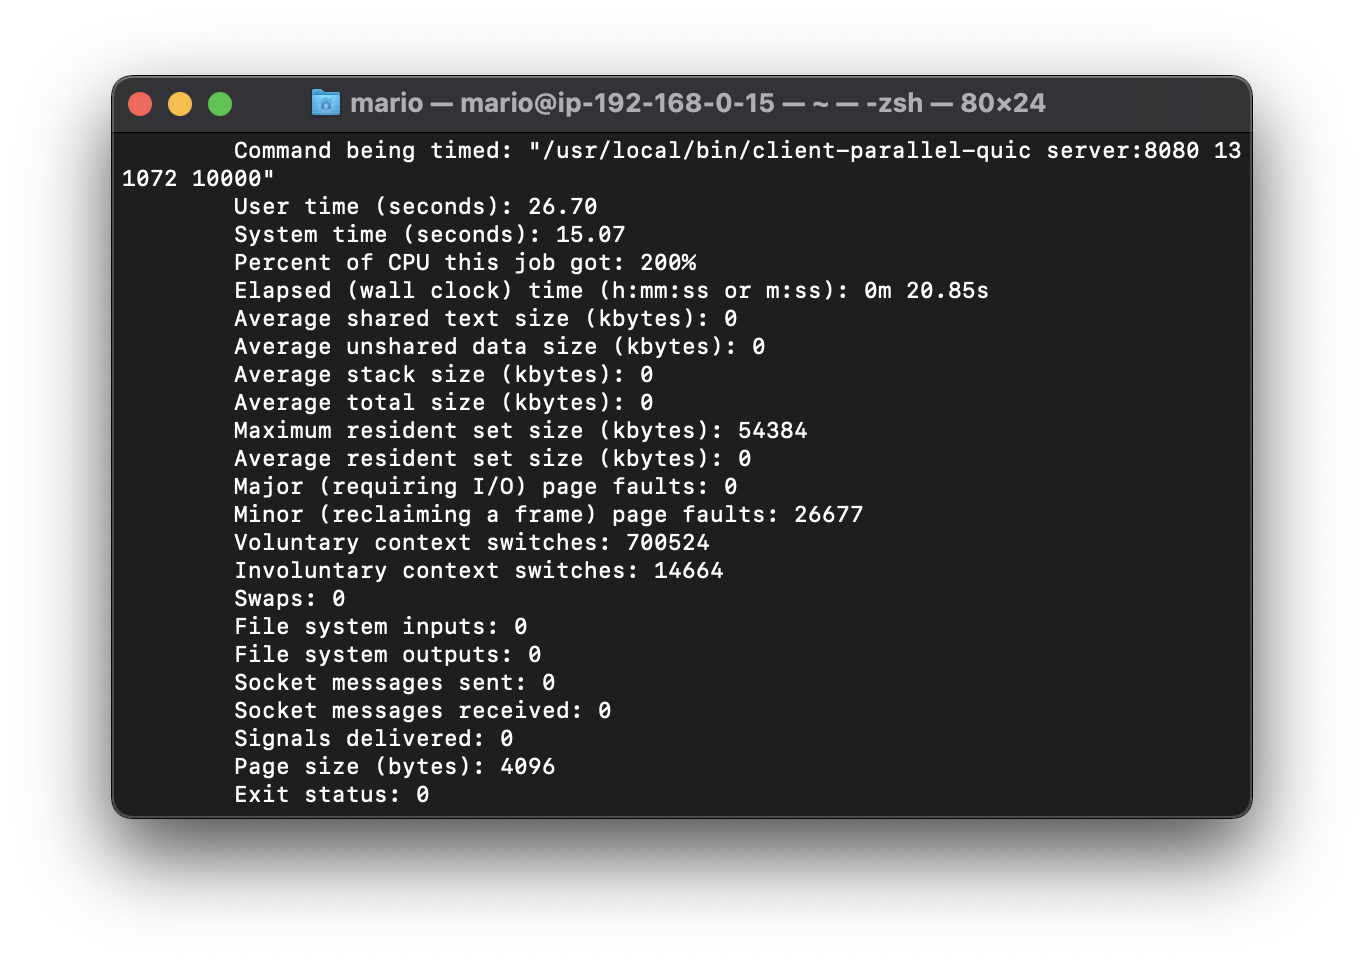
\includegraphics[width=\linewidth]{figures/time.png}
    \caption{\textit{time} command Result}
    \label{fig:time_command}
\end{figure}

The benchmark service itself is not enough to simulate a production environment, however. Therefore, all experiments are made inside a \gls{k8s} Cluster.

\subsubsection{K8s Cluster}

K8s is a production-grade container orchestrator, which is a common production environment used by most companies that have to deal with container management in the cloud. By choosing to use this environment allows easy networking setup for nodes running on different \gls{az}s. 

As every data center is always under the danger of downtime due to a natural disaster, running nodes on different \gls{az}s is a must have for companies that requires a disaster recovery plan. Therefore, enabling them to offer high availability services.

During the experiments, three scenarios are taken into account: when the client and server are running in the same node, when they are running in different nodes while in the same \gls{az}, and when they are running in different nodes while in different \gls{az}s. These are all possible scenarios when using \gls{k8s} on multiple \gls{az}s, since, depending on the configuration, applications may be running in any node.

K8s allows pod affinity and taint to be added to pod's configurations. This allows complete control over which pods are going to be scheduled to a specific node. Therefore, enabling all scenarios above to be possible.

During the \textit{Local} scenario, pod taint was used to make pods to be scheduled to a node in the same \gls{az}, and pod anti-affinity and affinity were used to make client and server pods to be scheduled to the same node. During the \textit{Single-\gls{az}} scenario, pod taint was also used to schedule pods to nodes in the same \gls{az}, but only pod anti-affinity was used to make sure there was only one pod running in each node. Finally, during the \textit{Multi-\gls{az}} scenario, pod taint was used to schedule pods to different \gls{az}s, while pod-affinity was also used to make sure there was only one pod running in each node.

The K8s cluster was deployed through the AWS EKS service. AWS allows easy setup with \textit{eksclt} command-line tool. Therefore, being able to quickly provide a cluster for experimenting.

\subsubsection{AWS}

\gls{aws} is one of the most popular cloud providers, offering a wide range of services. It was used as a provider due to its accessible price and since it met all experiments requirements.

Pricing was also taken into account when preparing for experiments. \gls{aws} not only charges for the \gls{ec2} instance and \gls{eks}, but also for data transfer between \gls{az}s, resulting in a hefty cost when exchanging terabytes of data.

During each experiment, 10000 requests are made. Therefore, one of the Multi-\gls{az} experiments, performing requests and responses with 512KiB payloads of a single protocol, transfers a total of 9.77 GiB of data. \gls{aws} charges \$0.02 per GiB transferred between \gls{az}s, resulting in an approximate cost of \$0.20 per experiment. With 9 protocols, ephemeral, sequential persistent, and parallel persistent clients, all Multi-\gls{az} experiments with 512KiB payloads costs approximately \$5.28 of data tranfer.

The payloads size is predetermined in compilation time. This value varies in the following manner: 2KiB, 8KiB, 32KiB, 128KiB, and 512KiB. These values were chosen due to cost and since they are a reasonable size of data transfer amongst services running in the cloud. Kafka's maximum package size’s default value is 1MB, because packages with more than 10MB can affect the performance of the cluster [25]. gRPC limits incoming messages size to 4MB to help prevent it from consuming excessive resources [26].

As each K8s node is an EC2 instance, it's important to choose carefully. The amount of CPU and memory can affect experiments. Therefore, it's required to choose a host with resources to avoid experiments to throttle.

Initial experiments were performed with the smallest \gls{ec2} instance type \textit{m6i.large} and \gls{k8s} pod's CPU limit was set to 1. However, QUIC ended up being throttled and required more resources to be able to perform correctly.

To avoid throttling, the \gls{cpu} limit was removed and the \gls{ec2} instance type was changed to \textit{m6i.xlarge}, which contains 2 \gls{cpu}s instead of 1. This assured pods to have all computational power it needs to perform correctly.

During QUIC's experiments, QUIC's Go implementation issued a warning about the \gls{udp} receive buffer size (Figure \ref{fig:udp_buffer_size_warning}). It contained a link recommending it to increase this value, since Linux places restrictions to \gls{udp} decreasing its throughput \cite{udp_buffer_size_warning}. Therefore, it was increased from 128KiB to 26MiB, more than the recommended amount.

\begin{figure}[h!]
    \centering
    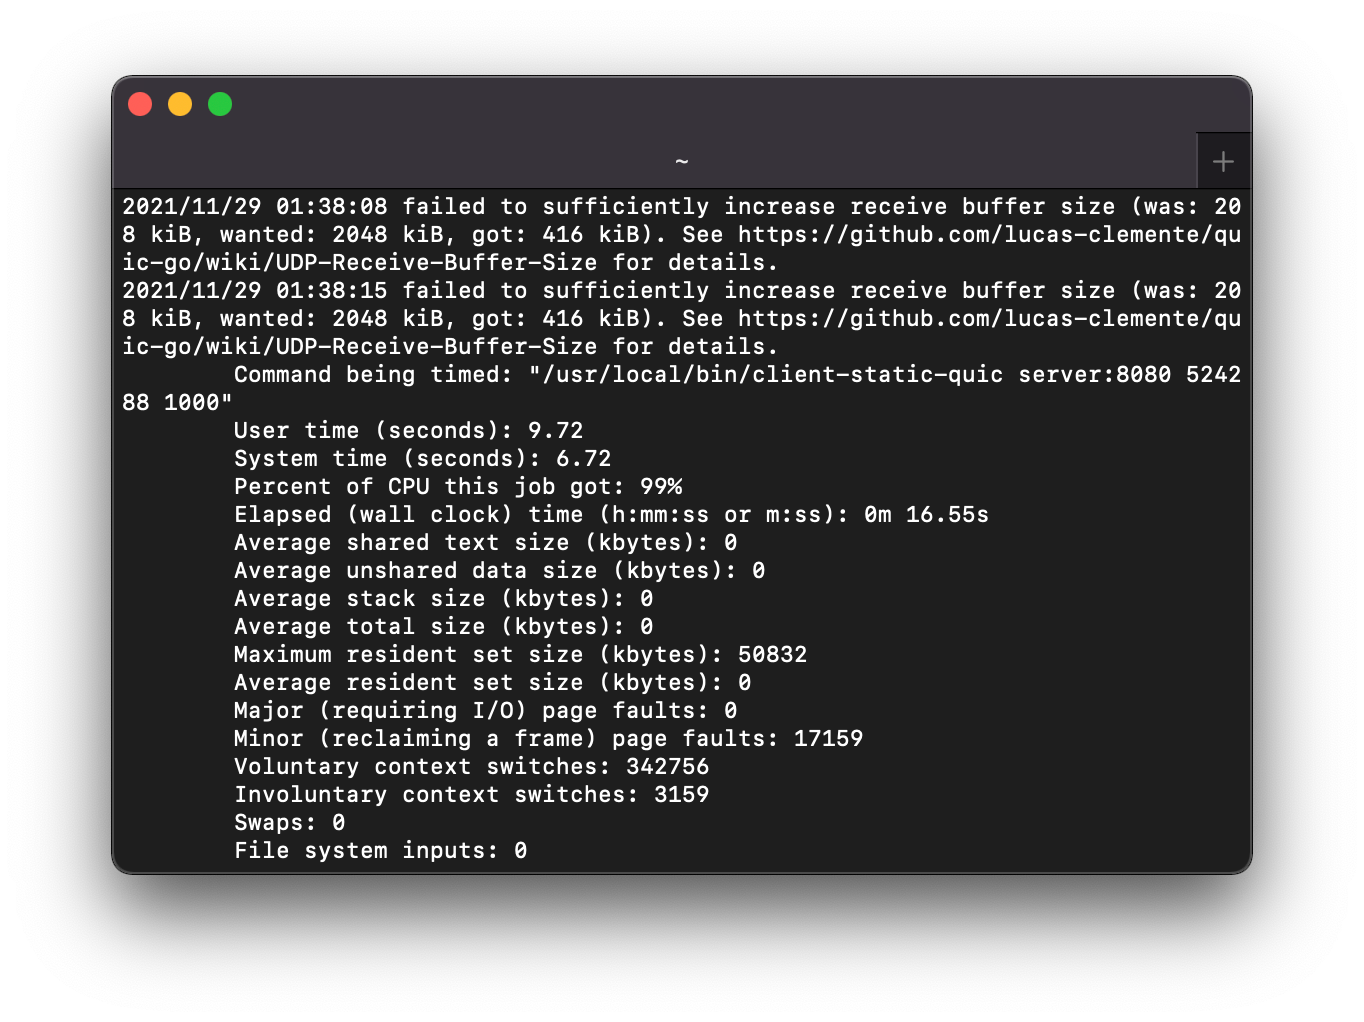
\includegraphics[width=\linewidth]{figures/quic_warning.png}
    \caption{\textit{quic-go} \gls{udp} Receive Buffer Size Warning}
    \label{fig:udp_buffer_size_warning}
\end{figure}

Additionally, \gls{az}s utilized during experiments were us-east-1a (use1-az1) and us-east-1b (use1-az2). The latter was only used during Multi-\gls{az} testing, while other experiments only used use1-az1.

\subsection{Execution}

Experiments execution is pretty straight forward. An even groups of nodes are created, and then a set of manifests is applied to the K8s Cluster. Thus, creating all necessary pods.

Clients and servers pods were allocated depending on the scenario being tested. \textit{Local} scenario requires one node, \textit{Single-\gls{az}} requires two nodes in the same \gls{az}, and \textit{Multi-\gls{az}} requires two nodes in different \gls{az}s. As this logic was incorporated into pods manifests, it's only a matter of patience to finish all experiments.

After experimentation and collecting metrics, node groups were deleted to make way to completely new node groups. This guarantees experiments are independent and don't affect one another.

\subsection{Summary}

This section explained the benchmark service, what kind of experiments were performed and how metrics were collected. It should be clear what kind of scenarios each experiment is trying to test and their objectives.

The following sections describes experiments results. It compares ephemeral and sequential persistent clients, and sequential persistent and parallel persistent clients. Consequently, putting each protocol to its limit to be able to show their benefits and drawbacks.